 \mysection{The Spriggan}{species-spriggan}

   \flavor{"Is it not enough?" he said in his strange rich magical voice, and pointed across his wide lands with the fingers that summoned wonder. ~\\ ~\\ She sighed: it was not enough. \Tilde Lord Dunsany} 

\begin{center}
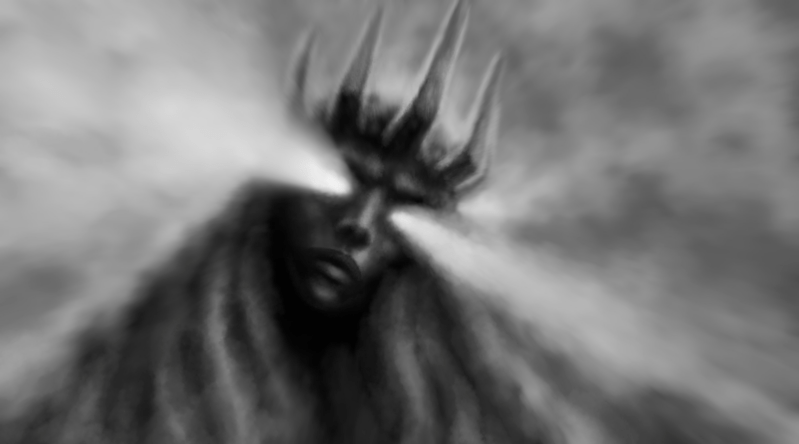
\includegraphics[width=\linewidth,keepaspectratio=true]{species/Spriggan1}
\end{center}

\begin{multicols*}{2}\raggedcolumns

  \mysubsection{Appearance}{spriggan-appearance}
  
  You hail from Elfland, beyond the reach of death.  Like your brothers and sisters the \Murk you are the Nomadic People, the Rom - cursed with curiosity and infected with the fire that burns in the hearts of the Hallowed to know more, to see the passage of time, and to breathe the air of decay.  All it cost was your soul.  

  You cannot find your way home again, for the bright line between this world and Elfland ebbs forever before you.  Wherever you are is where Elfland cannot be.

  Your bloodline allows you to strike bargains with the lowest of the Small Gods, the Forgotten who stand at the threshold of the void.  The fear of oblivion dominates every desire and scheme of these sanguinary spirits.  You steal them away from the doorway of nothingness and by Remembering them, allow them to touch reality once again.  In Remembering, you allow their souls to mingle inside of you, and sing through you - so that in the never-ending ache of the Mortal realm you might, for a moment, remember the feel of the heat of Elfin hearths and the smell of the lavender fields you dream of.  

  You are tall, lithe, and ethereal; Spriggan often stand over 2m, with leaf-shaped ears, long fingers, and gaunt faces vaguely reminiscent of deer or goats.  Older Spriggan often appear cadaverous - while you can't die from old age, your body begins to rot outside of the realm of Elfland (this has no effect on your powers).  Your skin and eye color is as varied as the Mortal races, and from a distance you might pass for human - except for the horns.  Some are small, barely noticeable stubs while other Spriggan sprout deer antlers, curling ram's horns, or tree branches.  It is not uncommon for birds to roost on your horns if they are well developed enough.


  \mysubsection{Creation}{spriggan-creation}

  \callout {
    \mynumlist {
        \item You start with \mybold{6 Flesh and 4 Grit}.
        \item Move your \AWA \DCUP (to a d6).
        \item If you need to \RS:\AWA, you only fail on a natural 1 (instead of a 1 or 2). Put a check next to \AWA on your \mylink{Adventurer Sheet}{adventurer-sheet.10} so you don't forget.
        \item Write down your \mylink{Virtues}{spriggan-virtues}.
        \item Write down your \mylink{Complication}{spriggan-complications}.
        \item Write down your \mylink{Starting Gear}{spriggan-starting-gear}.
    }
 }



  \mysubsection{Spriggan Virtues}{spriggan-virtues}

 \myhighlight{Sovereignty}{spriggan-virtues-sovereignty}

  Though you have been cast out of Elfland, the noble blood of the King of Elfland still runs through your veins.  You may use this sanguine supremacy to summon and command \mypg{the Abandoned}{forgotten-abandoned} and \mypg{the Obliterated}{forgotten-obliterated} (collectively known as \mybold{the Forgotten}), ghosts who live at the edge of oblivion.

The Abandoned are Small Gods whose names have disappeared from the tongues of men; they exist only as a line in a book buried by the sands of the deserts, etched on forgotten stela in the wilderness, or inscribed on scrimshaw lost beneath the waves.  When an Abandoned's name is finally lost, they become the Obliterated - totems and symbols of what they once were, raw power in the form of beasts (through the \mylink{Fealty of the Beasts}{forgotten-fealty-beasts}), elementals (through the \mylink{Fealty of the Elements}{forgotten-fealty-elements}), and devils (through the \mylink{Fealty of the Damned}{forgotten-fealty-damned}).


Your power over the Forgotten is manifest in your Sovereignty.  

\callout{You begin with a Sovereignty of 1, and your \MAX Sovereignty is 9.}
  

  \myhighlight{Remembrance of Elfland}{spriggan-virtues-remembrance-elfland}

  One of the names of the Abandoned exists in your memory. If you know which Abandoned you want to serve you when you first begin, you can name them immediately - otherwise, you can name them at any point in the campaign (when they hopefully appear in your time of need!). Once you name your Abandoned, you cannot change - it is as if you had always known its name, and suddenly remembered it. See the section on \mypg{The Abandoned}{forgotten-abandoned} for more info.


    
  \myhighlight{Fealty of the Beasts}{spriggan-virtues-fealty-beasts}

   You know the ways of summoning and commanding Sprites and more powerful zoological monsters. See the section \mylink{Fealty of the Beasts}{forgotten-fealty-beasts} under \mypg{Remembrance}{remembrance}

\myhighlight{Sword Magic}{spriggan-virtues-sword-magic}

  You know the wondrous ways of enchanting blades through \mypg{Sword Magic}{wonder-sword-magic}. 

  \myhighlight{Tongues}{spriggan-virtues-tongues}

  You know how to speak all \mypg{Idiolects and Dialects}{civilization-languages}.

  \myhighlight{Undreamt}{spriggan-virtue-undreamt}

  You stand outside of the Dream and are thus untouched by Sish, the Handmaiden of Time. You are immune to aging of any kind, and your \DEATH starts at Tough (d4).

\newpage

  \mysubsection{Complications}{spriggan-complications}

  \myhighlight{Alien}{spriggan-complication-alien}

  As far as Mortals are concerned, you are deeply and fundamentally \myital{weird}. You are eerie and alien, and it's not uncommon for other creatures to react to your presence with fear or loathing. Dogs bark at your approach, a cold breeze seems to follow you, you don't blink enough and your smile never seems to touch your eyes. You are one of the Rom, the Nomadic People - and there are no campfires where you will find welcome, save with your Band.

  \myhighlight{Antlers}{spriggan-complication-antlers}

  Antlers or tree branches grow from your head; birds often roost there (and if they do, you can speak with them). You can't wear helmets or use a \mylink{Bow}{gear-weapons} or \mylink{Strongbow}{gear-weapons}. You can't attack with your antlers, but you can sacrifice them for the same effect as wearing a \mylink{Helmet}{gear-armor}. Antlers will regrow during \mylink{Downtime}{downtime}.

  \myhighlight{Iron allergy}{spriggan-complication-iron-allergy}
    
    Prolonged bare-skin exposure to iron causes severe burns and painful blisters. Touching iron with your bare skin feels like picking up something uncomfortably hot; holding something made of iron for longer than a few Moments is impossible. If you are holding something made of iron with your bare hands, take 1 point of Flesh damage at the top of the next (and every following) Moment. 

  \myhighlight{Unseelie}{spriggan-complication-unseelie}
    
  You are creature of Chaos, one of the \mylink{Unseelie}{the-inhabitants} - and are thus \mybold{Unhallowed}.


  \mysubsection{Starting Gear}{spriggan-starting-gear}

  \callout{\footnotesize{
  You begin with:

  \mybullet {
    \item a pair of leather workgloves;
    \item two silver \mylink{Daggers}{gear-dex-weapons} OR a \mylink{Spear}{gear-vig-weapons}; 
    \item \UDD{d4} of \mylink{Personal Provisions}{gear-equipment};
    \item a set of prayer candles;
    \item a block of salt (for licking) and a pouch of dead mice;
    \item a pouch of 3 gems (roll on the \mylink{Gems table}{appendix-a-gems} in Appendix A)
    \item one pick OR 3 rolls on the \mylink{Random Items}{appendix-a-random-items} table in Appendix A;
  }
}}

    \myhighlight{What Next?}{spriggan-what-next}

    To better understand how you might command \mybold{the Forgotten},  read the chapter on \mypg{Remembrance}{remembrance}. You should also take a peek at how to make magical weapons through the Wonder of \mypg{Sword Magic}{wonder-sword-magic}.

\myimage{species/Spriggan2}

\end{multicols*}

